\newpage
\subsection{Introduction}
Nowadays, web applications are dominating online systems.
From Google, to Facebook and others, web applications are widely deployed across organizations and continuously accessed by end-users, both for their personal and professional daily tasks.
In practice, the development of these web applications heavily rely on a wide ecosystem of \emph{web frameworks}, which are intended to ease and foster the development process.
However, once deployed, the applications developed with such web frameworks do not exhibit the same performances, as reported by the \emph{Web Framework Benchmarks} periodically published by the \textsc{TechEmpower} company.\footnote{\url{https://www.techempower.com/benchmarks}}
Thanks to such benchmarks, developers can take informed decisions on the most performing technology to adopt to implement their web applications.
Unfortunately, one can regret that developers and benchmark providers focus mostly on popularity and performance criteria when picking a web framework, with less considerations for the resource consumption implications of their choice.
This is all the more regrettable that cloud providers are more and more adopted by developers to host these web applications.
While cloud providers offer a convenient elastic provision of resources to scale according to application requirements, this convenience may induce critical cost for their business.
% , their pricing model focuses on this resource consumption by charging the application owner.

Beyond the economical cost of web applications, one can also question the more global impact of web applications on worldwide carbon emissions.
Given the tremendous success of web applications, their deployment has severely increased over last years, thus causing a rebound effect on the power consumption of server infrastructure---being hosted or supported by cloud providers.
While one can challenge the relevance of features that are continuously deployed by developers to keep engaging end-users, reconciling economical and environmental concerns remains an open challenge to address.

Given this context, this paper intends to contribute to this challenge by investigating the energy footprint of web frameworks.
In particular, we aim to support the developers of web applications with relevant guidelines that can help them to choose the web framework that is not only the most popular or provide the best performances, but also exhibits a low energy footprint.
By minimizing the energy consumed to process user requests, with no service quality penalty, developers can reduce the operational cost of their web applications and contribute to reduce worldwide carbon emissions of ICT.
% While we assume this choice does not conflict with the appropriate selection of relevant user features, this topic remains out of the scope of this paper.

To achieve this objective, we leverage the \textsc{TechEmpower} \emph{Web Framework Benchmarks} to incorporate server-side energy measurements obtained from a software-defined power meter, named \textsc{PowerAPI}~\cite{}.
These measurements are then analyzed in depth to understand the key criteria that can amper the power consumption of web frameworks and derive guidelines to can help developers to pick the most energy efficient web frameworks according to their requirements.

The remainder of this paper is organized as follows.

\subsection{Comparaison between web frameworks}

Many studies have been conducted to compare the performance of web frameworks.

We can cite \cite{gajewski_analysis_2019} where they made a comparison between two of the most famous java frameworks, Play and Spring, or the work of \cite{benmoussa_new_2019} when they compare different PHP frameworks using 6 creterions intrinsic durability, industrialized solution, technical adaptability, strategy, technical architecture, and Speed, In the previous paper we find that all those 6 creterions have their own wait when it comes to choose which framework to take for a project. In our study we want to push a 7th criterion that impacts the economic outcome of the project.


\subsection{energy efficiency in software engineering}

In their paper \cite{pereira_energy_2017} the authors studied the impact of programming languages on energy, time, and Memory by using the CLBG benchmark,
where they executed 10 different benchmarks [ add citation] accross 27 wel-know programming languages [ add reference]
the work of the authors was an extension of the a research marled by [ add sitation[6 in the authers paper ]]. we continued  their work  with measuring the impact of programming languages choice in real life application instead of microbenchmark


Irene et al.\cite{manotas_investigating_2013} investigated the impact of web servers on energy when handleling web applications . they analysed 7 applications executed within 4 serveces with 38 different scenarios . the authors showed that the energy greatly depends on the web server , howerver the impact of the application may influence this energitical behaviour of the server.

In their approach they used measured the energy consumption during the integration tests and for us we measure with a simulation of a website when there is a client in another machine that requests the website, therefore we isolate the energy consumption of the server from the the client's one.


%notes 
% instead of focusing on energy or execution time we change the paradigm into efficiency and average power 
Other works have been done on the client side, as an example \cite{philippot_characterization_2014} as they concluded that theres is a variation among the different websites and the impact of the browser on this energy.



% \begin{longtable}{lll}
%     \toprule
%     framework        & language    & alternative implementations                        \\
%     \midrule
%     \endhead
%     \midrule
%     \multicolumn{3}{r}{{Continued on next page}}                                        \\
%     \midrule
%     \endfoot

%     \bottomrule
%     \endlastfoot
%     pico.v           & V           &                                                    \\
%     dylan            & Dylan       &                                                    \\
%     sinatra-sequel   & Ruby        & postgres passenger-mri postgres-passenger-mri...   \\
%     agoo             & Ruby        &                                                    \\
%     rack             & Ruby        & unicorn falcon                                     \\
%     h2o\_mruby       & Ruby        &                                                    \\
%     rails            & Ruby        & postgresql unicorn                                 \\
%     grape            & Ruby        & unicorn                                            \\
%     roda-sequel      & Ruby        & postgres passenger-mri postgres-passenger-mri...   \\
%     rack-sequel      & Ruby        & postgres passenger-mri postgres-passenger-mri...   \\
%     sinatra          & Ruby        & postgres passenger-mri postgres-passenger-mri...   \\
%     padrino          & Ruby        & unicorn                                            \\
%     ninglex          & Common Lisp &                                                    \\
%     ningle           & Common Lisp &                                                    \\
%     woo              & Common Lisp &                                                    \\
%     grails           & Groovy      &                                                    \\
%     hot              & Groovy      & mongodb postgres mysql                             \\
%     plack            & Perl        & async                                              \\
%     kelp             & Perl        & mongodb                                            \\
%     dancer           & Perl        &                                                    \\
%     mojolicious      & Perl        &                                                    \\
%     web-simple       & Perl        &                                                    \\
%     cowboy           & Erlang      &                                                    \\
%     elli             & Erlang      &                                                    \\
%     chicagoboss      & Erlang      &                                                    \\
%     mochiweb         & Erlang      &                                                    \\
%     opium            & OCaml       & haproxy                                            \\
%     morph            & OCaml       & static                                             \\
%     webmachine       & OCaml       & haproxy                                            \\
%     vertx-web-scala  & Scala       &                                                    \\
%     http4s           & Scala       &                                                    \\
%     akka-http        & Scala       & slick-postgres                                     \\
%     fintrospect      & Scala       &                                                    \\
%     finagle          & Scala       &                                                    \\
%     colossus         & Scala       &                                                    \\
%     finatra          & Scala       &                                                    \\
%     blaze            & Scala       &                                                    \\
%     play2-scala      & Scala       & netty anorm anorm-netty reactivemongo reactiv...   \\
%     finch            & Scala       &                                                    \\
%     scalene          & Scala       &                                                    \\
%     cask             & Scala       &                                                    \\
%     youi             & Scala       &                                                    \\
%     httpbeast        & Nim         &                                                    \\
%     prologue         & Nim         &                                                    \\
%     basolato         & Nim         &                                                    \\
%     jester           & Nim         &                                                    \\
%     falco            & F\#         &                                                    \\
%     frank            & F\#         &                                                    \\
%     suave            & F\#         &                                                    \\
%     giraffe          & F\#         & utf8json utf8direct stripped                       \\
%     zebra            & F\#         & simple                                             \\
%     vapor            & Swift       & fluent sql-kit postgres                            \\
%     swift-nio        & Swift       &                                                    \\
%     perfect          & Swift       & mysql postgresql mongodb                           \\
%     kitura           & Swift       & postgres postgres-orm postgres-orm-codable mo...   \\
%     racket           & Racket      &                                                    \\
%     vsgi             & Vala        &                                                    \\
%     valum            & Vala        &                                                    \\
%     wsgi             & Python      &                                                    \\
%     hug              & Python      &                                                    \\
%     crax             & Python      &                                                    \\
%     falcon           & Python      & py3 pypy2                                          \\
%     uvicorn          & Python      &                                                    \\
%     flask            & Python      & raw pypy pypy2 pypy2-raw nginx-uwsgi               \\
%     responder        & Python      &                                                    \\
%     klein            & Python      &                                                    \\
%     blacksheep       & Python      &                                                    \\
%     apidaora         & Python      & core                                               \\
%     bottle           & Python      & pypy2 raw nginx-uwsgi                              \\
%     japronto         & Python      &                                                    \\
%     api\_hour        & Python      & mysql json dbs plaintext                           \\
%     weppy            & Python      & py3 pypy2 nginx-uwsgi                              \\
%     starlette        & Python      &                                                    \\
%     emmett           & Python      &                                                    \\
%     sanic            & Python      &                                                    \\
%     aiohttp          & Python      & pg-raw                                             \\
%     tornado          & Python      & pypy2 postgresql-raw py3 py3-uvloop                \\
%     uwsgi            & Python      & nginx-uwsgi                                        \\
%     pyramid          & Python      & py2                                                \\
%     morepath         & Python      &                                                    \\
%     vibora           & Python      &                                                    \\
%     web2py           & Python      & optimized                                          \\
%     django           & Python      & postgresql                                         \\
%     cherrypy         & Python      & py3                                                \\
%     eve              & Python      &                                                    \\
%     webware          & Python      &                                                    \\
%     spyne            & Python      & raw nginx-uwsgi                                    \\
%     fastapi          & Python      & orjson                                             \\
%     quart            & Python      & uvicorn                                            \\
%     turbogears       & Python      &                                                    \\
%     m-web-server     & mumps       &                                                    \\
%     urweb            & Ur          & mysql cache mysql-cache                            \\
%     rouille          & Rust        &                                                    \\
%     warp-rust        & Rust        &                                                    \\
%     thruster         & Rust        &                                                    \\
%     ntex             & Rust        & db raw                                             \\
%     iron             & Rust        &                                                    \\
%     actix            & Rust        & core raw diesel pg                                 \\
%     roa              & Rust        & core tokio diesel pg sqlx                          \\
%     saphir           & Rust        &                                                    \\
%     may-minihttp     & Rust        &                                                    \\
%     rocket           & Rust        &                                                    \\
%     tokio-minihttp   & Rust        &                                                    \\
%     nickel           & Rust        &                                                    \\
%     hyper            & Rust        & db                                                 \\
%     gotham           & Rust        &                                                    \\
%     kooby            & Kotlin      &                                                    \\
%     pronghorn        & Kotlin      &                                                    \\
%     http4k           & Kotlin      & apache apache4 jetty ktorcio ktornetty netty ...   \\
%     ktor             & Kotlin      & jetty cio jasync reactivepg                        \\
%     hexagon          & Kotlin      & resin-mongodb jetty-postgresql resin-postgresql    \\
%     elixir-plug-ecto & Elixir      &                                                    \\
%     phoenix          & Elixir      &                                                    \\
%     fiber            & Go          & prefork                                            \\
%     webgo            & Go          &                                                    \\
%     gnet             & Go          &                                                    \\
%     goframe          & Go          &                                                    \\
%     revel            & Go          & fast raw jet qbs                                   \\
%     echo             & Go          &                                                    \\
%     gramework        & Go          &                                                    \\
%     gin              & Go          & scratch                                            \\
%     atreugo          & Go          & prefork                                            \\
%     beego            & Go          & orm-mysql                                          \\
%     kami             & Go          &                                                    \\
%     falcore          & Go          &                                                    \\
%     goji             & Go          &                                                    \\
%     clevergo         & Go          &                                                    \\
%     fasthttp         & Go          & prefork                                            \\
%     aah              & Go          & mysql postgresql                                   \\
%     gearbox          & Go          & prefork                                            \\
%     martini          & Go          &                                                    \\
%     go               & Go          & pgx pgx-easyjson pgx-quicktemplate pgx-prefor...   \\
%     evio             & Go          & stdlib                                             \\
%     chi              & Go          & scratch prefork gojay gojay-prefork sjson sjs...   \\
%     warp             & Haskell     & hasql mysql-haskell                                \\
%     yesod            & Haskell     & mongodb-raw                                        \\
%     wizzardo-inline  & Haskell     &                                                    \\
%     snap             & Haskell     &                                                    \\
%     spock            & Haskell     &                                                    \\
%     ihp              & Haskell     &                                                    \\
%     servant          & Haskell     & beam psql-simple                                   \\
%     stream           & Dart        &                                                    \\
%     start            & Dart        &                                                    \\
%     angel            & Dart        & postgres                                           \\
%     redstone         & Dart        & mongodb                                            \\
%     dart             & Dart        &                                                    \\
%     aqueduct         & Dart        &                                                    \\
%     aspcore-vb-mw    & VB          & ado-pg ado-my                                      \\
%     spider-gazelle   & Crystal     &                                                    \\
%     toro             & Crystal     &                                                    \\
%     onyx             & Crystal     &                                                    \\
%     h2o.cr           & Crystal     &                                                    \\
%     kemal            & Crystal     & concurrent-queries                                 \\
%     lucky            & Crystal     &                                                    \\
%     crystal          & Crystal     & radix                                              \\
%     grip             & Crystal     &                                                    \\
%     orion            & Crystal     &                                                    \\
%     amber            & Crystal     &                                                    \\
%     raze             & Crystal     &                                                    \\
%     collie           & D           & ldc                                                \\
%     vibed            & D           & dmd-pgsql ldc ldc-pgsql                            \\
%     hunt             & D           &                                                    \\
%     macchiato        & Clojure     &                                                    \\
%     aleph            & Clojure     &                                                    \\
%     luminus          & Clojure     &                                                    \\
%     pedestal         & Clojure     &                                                    \\
%     compojure        & Clojure     & raw                                                \\
%     http-kit         & Clojure     & raw                                                \\
%     duct             & Clojure     & mongodb httpkit aleph immutant                     \\
%     reitit           & Clojure     & jdbc async                                         \\
%     nestjs           & TypeScript  & mysql mongo fastify fastify-mysql fastify-mongo    \\
%     typescript-rest  & TypeScript  &                                                    \\
%     deno             & TypeScript  &                                                    \\
%     dropwizard       & Java        & mongodb postgres jdbi-postgres                     \\
%     httpserver       & Java        & postgres                                           \\
%     quarkus          & Java        & pgclient                                           \\
%     jooby            & Java        & netty jaxrs jetty pgclient                         \\
%     undertow         & Java        & postgresql                                         \\
%     tapestry         & Java        &                                                    \\
%     vertx-web        & Java        & mongodb postgres susom-postgres                    \\
%     jlhttp           & Java        & postgres                                           \\
%     voovan           & Java        &                                                    \\
%     play2-java       & Java        & netty ebean-hikaricp ebean-hikaricp-netty jpa...   \\
%     officefloor      & Java        & raw tpr micro thread\_affinity netty spring\_data  \\
%     jersey           & Java        &                                                    \\
%     proteus          & Java        & mysql                                              \\
%     light-4j         & Java        &                                                    \\
%     activeweb        & Java        & jackson                                            \\
%     minijax          & Java        &                                                    \\
%     jetty            & Java        & servlet                                            \\
%     spark            & Java        &                                                    \\
%     grizzly          & Java        & jersey                                             \\
%     servlet          & Java        & lib-native mysql postgresql                        \\
%     tio-mvc          & Java        &                                                    \\
%     baratine         & Java        &                                                    \\
%     servicetalk      & Java        &                                                    \\
%     play1            & Java        &                                                    \\
%     ninja-standalone & Java        &                                                    \\
%     nanohttpd        & Java        &                                                    \\
%     simple-server    & Java        &                                                    \\
%     restexpress      & Java        & mysql-raw                                          \\
%     javalin          & Java        &                                                    \\
%     jawn             & Java        &                                                    \\
%     redkale          & Java        & postgres                                           \\
%     revenj-jvm       & Java        &                                                    \\
%     spring-webflux   & Java        & mongo pgclient rxjdbc jdbc                         \\
%     firenio          & Java        & http-lite                                          \\
%     curacao          & Java        &                                                    \\
%     bayou            & Java        &                                                    \\
%     wizzardo-http    & Java        &                                                    \\
%     netty            & Java        &                                                    \\
%     armeria          & Java        &                                                    \\
%     vertx            & Java        & postgres                                           \\
%     comsat           & Java        & servlet-undertow webactors-netty webactors-un...   \\
%     ratpack          & Java        & jdbc pgclient                                      \\
%     wicket           & Java        &                                                    \\
%     wildfly-ee       & Java        &                                                    \\
%     undertow-jersey  & Java        & hikaricp                                           \\
%     micronaut        & Java        &                                                    \\
%     servlet3         & Java        & sync                                               \\
%     act              & Java        & hibernate-pgsql hibernate-pgsql-rythm hiberna...   \\
%     blade            & Java        &                                                    \\
%     rapidoid         & Java        & mysql postgres http-fast                           \\
%     smart-socket     & Java        &                                                    \\
%     gemini           & Java        & mysql postgres                                     \\
%     greenlightning   & Java        &                                                    \\
%     helidon          & Java        &                                                    \\
%     spring           & Java        & jpa mongo                                          \\
%     codeigniter      & PHP         &                                                    \\
%     fat-free         & PHP         & raw                                                \\
%     php              & PHP         & activerecord raw7-tcp pgsql-raw h2o unit pool...   \\
%     cakephp          & PHP         &                                                    \\
%     ubiquity         & PHP         & workerman swoole swoole-mysql roadrunner road...   \\
%     fuel             & PHP         &                                                    \\
%     sw-fw-less       & PHP         &                                                    \\
%     hyperf           & PHP         & raw micro                                          \\
%     kumbiaphp        & PHP         & raw workerman workerman-mysql                      \\
%     workerman        & PHP         & pgsql async                                        \\
%     lumen            & PHP         & swoole                                             \\
%     peachpie         & PHP         &                                                    \\
%     yii2             & PHP         & raw                                                \\
%     php-ngx          & PHP         & mysql pgsql async                                  \\
%     laravel          & PHP         & swoole                                             \\
%     symfony          & PHP         & raw swoole                                         \\
%     imi              & PHP         & query-builder raw                                  \\
%     webman           & PHP         &                                                    \\
%     phalcon          & PHP         & mongodb micro                                      \\
%     slim             & PHP         &                                                    \\
%     amp              & PHP         &                                                    \\
%     hhvm             & PHP         &                                                    \\
%     spiral           & PHP         &                                                    \\
%     swoole           & PHP         & postgres no-async                                  \\
%     hamlet           & PHP         & swoole workerman                                   \\
%     simps            & PHP         & micro                                              \\
%     one              & PHP         &                                                    \\
%     zend             & PHP         &                                                    \\
%     phpixie          & PHP         &                                                    \\
%     comet            & PHP         & mysql                                              \\
%     nginx            & C           &                                                    \\
%     onion            & C           &                                                    \\
%     duda             & C           &                                                    \\
%     libreactor       & C           & server                                             \\
%     lwan             & C           & lua                                                \\
%     h2o              & C           &                                                    \\
%     facil\_io        & C           &                                                    \\
%     octane           & C           &                                                    \\
%     polkadot         & JavaScript  & mysql postgres mongodb                             \\
%     restify          & JavaScript  &                                                    \\
%     hapi             & JavaScript  & nginx mysql postgres                               \\
%     nodejs           & JavaScript  & chakra mongodb mongodb-raw mysql postgres          \\
%     restana          & JavaScript  &                                                    \\
%     es4x             & JavaScript  &                                                    \\
%     sailsjs          & JavaScript  & postgres                                           \\
%     just             & JavaScript  &                                                    \\
%     fastify          & JavaScript  & mysql postgres                                     \\
%     ringojs          & JavaScript  & convenient                                         \\
%     express          & JavaScript  & chakra mongodb mysql postgres graphql-mysql g...   \\
%     koa              & JavaScript  & mysql postgres                                     \\
%     0http            & JavaScript  &                                                    \\
%     openresty        & Lua         &                                                    \\
%     octopus          & Lua         &                                                    \\
%     lapis            & Lua         &                                                    \\
%     easyrpc          & C\#         &                                                    \\
%     aspcore-mono     & C\#         & pg mw mw-pg mw-my mvc mvc-pg mvc-my                \\
%     servicestack     & C\#         &                                                    \\
%     tetsuweb         & C\#         &                                                    \\
%     beetlex          & C\#         & core core-updb debug                               \\
%     aspcore          & C\#         & pgo ado-pg ado-pg-up pgo-pg pgo-pg-up mw mw-j...   \\
%     revenj           & C\#         &                                                    \\
%     carter           & C\#         &                                                    \\
%     aspnet-mono-ngx  & C\#         & jn ss my my-ef                                     \\
%     genhttp          & C\#         &                                                    \\
%     ben              & C\#         & pg                                                 \\
%     evhttp-sharp     & C\#         &                                                    \\
%     zysocket-v       & C\#         &                                                    \\
%     nancy            & C\#         & netcore                                            \\
%     aspcore-corert   & C\#         &                                                    \\
%     cuehttp          & C++         &                                                    \\
%     libhttpserver    & C++         &                                                    \\
%     ffead-cpp        & C++         & mongo-raw lithium cinatra drogon libreactor h...   \\
%     lithium          & C++         & postgres postgres-batch                            \\
%     wt               & C++         & postgres                                           \\
%     treefrog         & C++         & postgres mongodb                                   \\
%     ulib             & C++         & plaintext\_fit json json\_fit mysql postgres po... \\
%     cppcms           & C++         & postgres                                           \\
%     oatpp            & C++         & no-mp async async-no-mp                            \\
%     poco             & C++         &                                                    \\
%     silicon          & C++         &                                                    \\
%     cutelyst         & C++         & pf-apg pf-pg pf-my thread thread-apg thread-p...   \\
%     drogon           & C++         & core                                               \\
%     cinatra          & C++         &                                                    \\
%     libsniper        & C++         &                                                    \\
%     cpoll\_cppsp     & C++         & raw postgres-raw postgres-raw-threadpool           \\
% \end{longtable}


\newcommand\duration{20}
\newcommand\parallelclient{512}
\section{Experimental Protocol}

In this section, we describe the environement used during the experiments covering hardware material, experiments of the framework and the methodology.

\subsection{experiment workflow}
To mesure compare the energy consumption and performance effeciency between mutiple frameworks, each framework used to implement the samewebsite answering the same urls and requesting the same database. Then we run the same algorthim for all impelentations.
\begin{enumerate}
    \item lunch the framework
    \item wait for \duration s for the warmup
    \item measure the average power when the framework is in idle state
    \item using multiple clients. we send the same request in simultaneously during \duration s
    \item increase the number of parallel request
    \item measure the enrgy during this execution
    \item change the request type
    \item repeat from 3 rd step
\end{enumerate}
the section will detail each type of experiments  and the purpose behind it giving some examples of the expecteed response

\subsection{Test categories }
We have 6 categories of tests :

\subsubsection{Idle}
In this test we measure the idle energy consumption of the framework: this reflects the average energy consumption of an application during the periods when we have no clients.
For example, a company website beyond working hours or a small website at night.


\subsubsection{Single query}
During this test, each request  is processed by fetching a single row from a simple database table. That row is then serialized as a JSON response.

\subsubsection{Multiple queries}
this test aims to test the behaviour of a framework when it process multiple entries from the database.
Therefore each request is processed by fetching multiple rows from a simple database table and serializing these rows as a JSON response.
%The test is run multiple times: testing 1, 5, 10, 15, and 20 queries per request. All tests are run at 512 concurrency.
%//TODO  add the cuncurency levels 
% \subsubsection{Cached queries}
% To evaluate the performance of a framework when the data is already cashed  each request is processed by fetching multiple cached objects from an in-memory database and serializing these objects as a JSON response.
%  The test is run multiple times: testing 1, 5, 10, 15, and 20 cached object fetches per request. All tests are run at 512 concurrency. Conceptually, this is similar to the multiple-queries test except the fact that it uses a caching layer.
\subsubsection{Fortunes}
In this test, the framework's ORM is used to fetch all rows from a database table containing an unknown number of Unix fortune cookie messages (the table has 12 rows, but the code cannot have foreknowledge of the table's size). An additional fortune cookie message is inserted into the list at runtime and then the list is sorted by the message text. Finally, the list is delivered to the client using a server-side HTML template. The message text must be considered untrusted and properly escaped and the UTF-8 fortune messages must be rendered properly.
% maybe i should remove it 
% \begin{listing}[language=html]
%     HTTP/1.1 200 OK
%     Content-Length: 1196
%     Content-Type: text/html; charset=UTF-8
%     Server: Example
%     Date: Wed, 17 Apr 2013 12:00:00 GMT

%     <!DOCTYPE html><html><head><title>Fortunes</title></head><body><table><tr><th>id</th><th>message</th></tr><tr><td>11</td><td>\&lt;script\&gt;alert(\&quot;This should not be displayed in a browser alert box.\&quot;);\&lt;/script\&gt;</td></tr><tr><td>4</td><td>A bad random number generator: 1, 1, 1, 1, 1, 4.33e+67, 1, 1, 1</td></tr><tr><td>5</td><td>A computer program does what you tell it to do, not what you want it to do.</td></tr><tr><td>2</td><td>A computer scientist is someone who fixes things that aren\&apos;t broken.</td></tr><tr><td>8</td><td>A list is only as strong as its weakest link. — Donald Knuth</td></tr><tr><td>0</td><td>Additional fortune added at request time.</td></tr><tr><td>3</td><td>After enough decimal places, nobody gives a damn.</td></tr><tr><td>7</td><td>Any program that runs right is obsolete.</td></tr><tr><td>10</td><td>Computers make very fast, very accurate mistakes.</td></tr><tr><td>6</td><td>Emacs is a nice operating system, but I prefer UNIX. — Tom Christaensen</td></tr><tr><td>9</td><td>Feature: A bug with seniority.</td></tr><tr><td>1</td><td>fortune: No such file or directory</td></tr><tr><td>12</td><td>hello world</td></tr></table></body></html>
% \end{listing}
\subsubsection{Update queries}

This test exercises database writes. Each request is processed by fetching multiple rows from a simple database table, converting the rows to in-memory objects, modifying one attribute of each object in memory, updating each associated row in the database individually, and then serializing the list of objects as a JSON response.
%  The test is run multiple times: testing 1, 5, 10, 15, and 20 updates per request. It is important that the number of statements per request is twice the number of updates since each update is paired with one query to fetch the object. All tests are run at 512 concurrency.

The response is analogous to the multiple-query test.

\subsubsection{Plain text}
In this test, the framework responds with the simplest of responses: a "Hello, World" message rendered as plain text. The size of the response is kept small so that gigabit Ethernet is not the limiting factor for all implementations. HTTP pipelining is enabled and higher client-side concurrency levels are used for this test.

\subsubsection{JSON Serialization}
In this test, each response is a JSON serialization of a freshly-instantiated object that maps the key message to the value "Hello, World!"



\subsection{Architecture}
The aim is to compare the energy consumption of different frameworks. For this we consider the framework as a blackbox and we take into account the response to the 6 previous requests using the same database.
In order to isolate the energy consumption of the framework the test is run in a seperate machine with the minimum services and the powermeter.
Figure \ref{fig:architecture} illustrates the architecture of our system

\begin{figure}\centering
    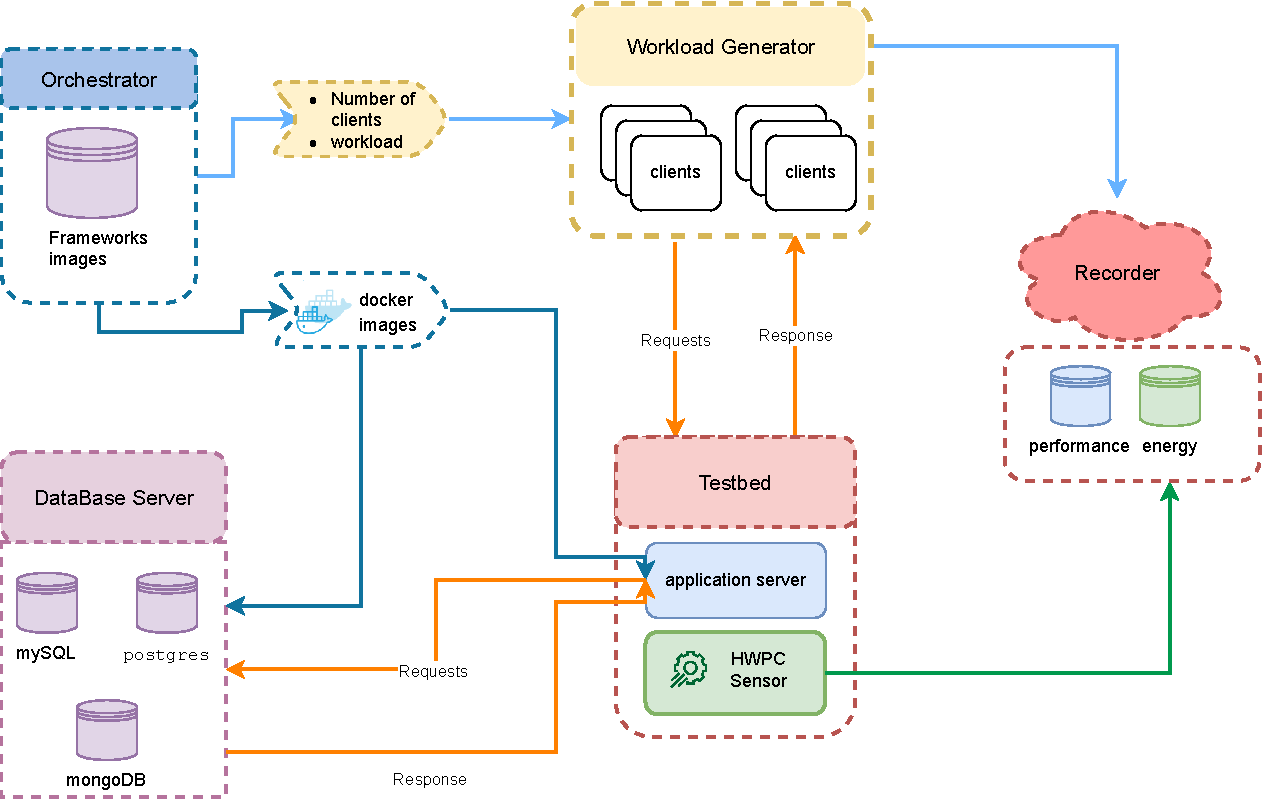
\includegraphics[width=.8\columnwidth]{imgs/architecture}
    \caption[Architecture]{Architecture of the experiments}
    \label{fig:architecture}
\end{figure}

\begin{itemize}
    \item orchestrator : the part that is responisble for creating docker images, selecting the benchmarks and launching the tests;
    \item web server : or the system under test (SUT) is the machine  responsible for launching the framework  by means of the pre-installed powermeter;
    \item database server : a offers the same data base that will be used by all the frameworks during the tests
          %(is seperated from the application server to neglect its contribution in energy calculation?) 
    \item client machines : To avoid the bottleneck on the client's side, client requests are sent from another machine (one or many) that simulates hundreds of concurrent connections to the framework.
          %Does even one machine simulate hundreds? 
    \item recorder : the party responsible for collecting the power data from the SUT and the performance metrics collected by the clients \todo{add link to the measurement process}
\end{itemize}

The tests have been executed in machines from the cluster chetemi of the \reference{Grid500} plateform .
\todo{add hardware description}

\paragraph{Note}
It has been proven in {cite } that docker does not influence on the energy cosumption. Thus, using its containers and isolation allow to avoid any alteration of the operation system after testing one benchmark and to take advantage of its reproducibility.

\subsection{Measurement Workflow}
We focus on comparing the energitical behaviour of different frameworks in multiple scenarios

To measure the energy consumption of those frameworks, we launch each one for a fixed duration, then all the clients send multiple requests simultaneously.
We calculate %calculate - with paper and pen or calculator, compute - with computer (programs)
the number of satisfied responses which reflects the performance of the framework, the average latency and the global energy consumed during the whole period to deduce the energy cost of each request.


\subsubsection{Runtime Measurements}
\begin{itemize}
    \item energy measurement :
          we use \reference{powerapi}, a software powermeter  to gather the runninng power of the SUT, after we project the timestamps of each experiment phase to calculate the energy consumption of the framework during this phase.
          Energy is an integral of power over time, so we use a numerical apporoach to estimate this energy. \todo{add formula}
          after this we devide the calculated energy per number of responses
          during this phase
          we have 4 mertrics :

    \item Total cost of the energy during each period
    \item Total number of requests
    \item Average latency
    \item Average energy cost per request
\end{itemize}


\subsubsection{Bias analysis}
we are aware of bias analysis regarding the estimation of the total energy cost , the interference of other system processess during the execution and some external events. Thus, we run experiments multiple times and compute the average.

\subsection{tools }
